\chapter{Hecke Operators as Random Walks on Trees}\label{ch:07}

In 1959 Harry Kesten computed the probability that a symmetric random walk on a free group returns to its starting point, and found that it decays exponentially, like $\rho^n$ with $\rho<1$ up to a polynomial factor \cite{kesten1959}. The work of Ihara on discrete subgroups of $\PGL_2(\Q_q)$ and Serre's lectures on trees \cite{ihara1966,serre1980} identified the regular tree on which such a walk lives with the Bruhat Tits tree of $\PGL_2(\Q_q)$, on which the Hecke operator $T_q$ of the theory of modular forms acts as the adjacency operator. In 1981 McKay found Kesten's spectral law again as the limiting eigenvalue distribution of large random regular graphs \cite{mckay1981}, and in 1997 Serre found it once more as the limiting distribution of the eigenvalues of $T_q$ on spaces of modular forms of growing level or weight \cite{serre1997}. This chapter explains why these are one law. We prove the tree theorem (Theorem~\ref{thm:07tree}), state the vertical Sato Tate theorem with a probabilistic proof idea, and test it on supersingular isogeny graphs at $207$ prime levels.

\section{The Bruhat Tits tree}\index{Bruhat Tits tree}

Fix a prime $q$. A lattice in $\Q_q^2$ is a $\Z_q$ submodule $\Z_qu\oplus\Z_qv$ spanned by a basis $u,v$ of $\Q_q^2$, and two lattices $L,L'$ are homothetic if $L'=cL$ for some $c\in\Q_q^\times$. The vertices of $\T_q$ are homothety classes $[L]$. Two classes are joined by an edge if they have representatives with $qL\subsetneq L'\subsetneq L$. Since $L/qL\cong\mathbb{F}_q^2$ has exactly $q+1$ lines, every vertex has $q+1$ neighbours, and one shows that the resulting graph is connected and has no cycles, so $\T_q$ is the $(q+1)$ regular tree \cite{serre1980}. The group $\GL_2(\Q_q)$ acts on lattices, the centre acts trivially on classes, and $\PGL_2(\Q_q)$ acts on $\T_q$ by automorphisms, transitively on vertices, with the stabiliser of $[\Z_q^2]$ equal to $\PGL_2(\Z_q)=\GL_2(\Z_q)/\Z_q^\times$, a maximal compact subgroup. Thus the vertex set is $\PGL_2(\Q_q)/\PGL_2(\Z_q)$, and functions on vertices are right $\PGL_2(\Z_q)$ invariant functions on the group.

If $L'\subseteq L$ and $L/L'\cong\Z/q^a\oplus\Z/q^b$ with $a\ge b$, then $d([L],[L'])=a-b$. For $n\ge1$ the sphere $\{w:d(v,w)=n\}$ around a vertex $v$ has $(q+1)q^{n-1}$ elements.

\subsection{Hecke operators}\index{Hecke operator}

The Hecke operator $T_q$ acts on functions on lattice classes by $T_qf([L])=\sum f([L'])$, summed over the $q+1$ sublattices of index $q$. This is the adjacency operator $A$ of $\T_q$. More generally let $A_n$ be the operator $A_nf(v)=\sum_{d(v,w)=n}f(w)$, with $A_0=I$; equivalently $A_n(v,w)$ counts nonbacktracking walks of length $n$ from $v$ to $w$, since on a tree such a walk is a geodesic and there is exactly one between vertices at distance $n$.\index{nonbacktracking operator} The classical Hecke operator $T_{q^n}$ sums over all sublattices of index $q^n$; each of them is $q^bL''$ with $L/L''$ cyclic of order $q^{n-2b}$, so on classes $T_{q^n}=A_n+A_{n-2}+A_{n-4}+\cdots$ (Exercise~\ref{ex:07hecke}). All these operators commute: they lie in the spherical Hecke algebra, which is the polynomial algebra $\C[T_q]$.

\section{The tree theorem}

Let $o$ be a fixed vertex and let $\mu_q$ be the spectral measure of the bounded self adjoint operator $X=q^{-1/2}A$ on $\ell^2(\T_q)$ at $\delta_o$, so that $\langle\delta_o,\phi(X)\delta_o\rangle=\int\phi\,d\mu_q$ for continuous $\phi$. Write $U_n$ for the Chebyshev polynomials of the second kind, $U_n(\cos\theta)=\sin((n+1)\theta)/\sin\theta$, and recall from Chapter~\ref{ch:04} that the $U_n(x/2)$ are orthonormal for the Sato Tate measure $\ST(dx)=\sqrt{4-x^2}\,dx/(2\pi)$ on $[-2,2]$.

\begin{theorem}[Tree theorem, this book]\label{thm:07tree}\index{Kesten McKay law}
Let $q\ge2$ be an integer, let $\T_q$ be the $(q+1)$ regular tree, and put $B_n=q^{-n/2}A_n$.
\begin{enumerate}
\item $B_1=U_1(X/2)$ and $B_n=U_n(X/2)-q^{-1}U_{n-2}(X/2)$ for $n\ge2$.
\item $c_n=\int U_n(x/2)\,d\mu_q(x)$ equals $q^{-n/2}$ for $n$ even and $0$ for $n$ odd.
\item $\mu_q$ is supported on $[-2,2]$ with the Kesten McKay density
\[
\mu_q(dx)=\frac{q+1}{(q^{1/2}+q^{-1/2})^2-x^2}\cdot\frac{\sqrt{4-x^2}}{2\pi}\,dx .
\]
\item If $S$ is simple random walk on $\T_q$ started at $o$, then for $m\ge0$
\[
\int x^{2m}\,d\mu_q=(q+1)^{2m}q^{-m}\Prob(S_{2m}=o).
\]
\item The walk returns to $o$ with probability $1/q$, and the Green function $G(1)=\sum_{n\ge0}\Prob(S_n=o)$, the expected number of visits to $o$, equals $q/(q-1)$.\index{Green function}
\item $\mu_q\Rightarrow\ST$ weakly as $q\to\infty$.
\end{enumerate}
\end{theorem}

\begin{proof}
(1) A vertex at distance $n\ge1$ from $w$ has one neighbour at distance $n-1$ and $q$ neighbours at distance $n+1$, while $w$ itself has $q+1$ neighbours at distance $1$. For $n\ge1$ the entry $(AA_n)(v,w)$ counts the neighbours of $v$ at distance $n$ from $w$, so it is $1$ if $d(v,w)=n+1$, $q$ if $d(v,w)=n-1\ge1$, $q+1$ if $n=1$ and $v=w$, and $0$ otherwise. Hence
\[
AA_1=A_2+(q+1)I,\qquad AA_n=A_{n+1}+qA_{n-1}\quad(n\ge2).
\]
Dividing by $q^{(n+1)/2}$, $XB_1=B_2+(1+q^{-1})I$ and $XB_n=B_{n+1}+B_{n-1}$ for $n\ge2$. The Chebyshev recursion $xU_n(x/2)=U_{n+1}(x/2)+U_{n-1}(x/2)$, with $U_0=1$ and $U_1(x/2)=x$, gives $B_1=X=U_1(X/2)$ and
\[
B_2=XU_1(X/2)-(1+q^{-1})I=U_2(X/2)-q^{-1}U_0(X/2).
\]
For $n\ge2$ the recursion $B_{n+1}=XB_n-B_{n-1}$ is linear and is satisfied separately by the sequences $U_n(X/2)$ and $q^{-1}U_{n-2}(X/2)$; since the formula holds for $n=2$ and, with the convention $U_{-1}=0$, also for $n=1$, induction proves (1).

(2) The tree has no cycles, so a nonbacktracking walk of positive length never returns: $\langle\delta_o,B_n\delta_o\rangle=0$ for $n\ge1$. Taking the $(o,o)$ entry of (1) gives $c_1=0$ and $c_n=q^{-1}c_{n-2}$ for $n\ge2$, and $c_0=1$. Hence $c_{2m}=q^{-m}$ and $c_{2m+1}=0$.

(3) Put $R=(q+1)/\sqrt q$, so that $\mu_q$ lives on $[-R,R]$ because $\|X\|\le R$. Since $\sum_nc_n^2<\infty$, the series $f=\sum_nc_nU_n(x/2)$ converges in $L^2(\ST)$. With $x=2\cos\theta$ and $U_{2m}(\cos\theta)=\sum_{|j|\le m}e^{2ij\theta}$, summing over $m\ge|j|$ first (the double series converges absolutely),
\[
\begin{aligned}
f&=\sum_{m\ge0}q^{-m}\sum_{|j|\le m}e^{2ij\theta}=\frac{q}{q-1}\sum_{j\in\Z}q^{-|j|}e^{2ij\theta}\\
&=\frac{q+1}{q}\cdot\frac{1}{1-2q^{-1}\cos2\theta+q^{-2}},
\end{aligned}
\]
a Poisson kernel. Since $2\cos2\theta=x^2-2$, the denominator equals $q^{-1}\bigl((q^{1/2}+q^{-1/2})^2-x^2\bigr)$, which gives the stated density, positive and bounded on $[-2,2]$. The measure $f\,d\ST$ has Chebyshev moments $c_n$ by orthonormality, hence the same moments $\int x^k$ as $\mu_q$, because the $U_n(x/2)$ span the polynomials. Both laws live on $[-R,R]$, so they coincide by Theorem~\ref{thm:A:moments}. In particular $\mu_q$ is supported on $[-2,2]$.

(4) By definition $\int x^{2m}\,d\mu_q=q^{-m}A^{2m}(o,o)$, and $A^{2m}(o,o)$ is the number of closed walks of length $2m$ at $o$, each of which simple random walk follows with probability $(q+1)^{-2m}$.

(5) Let $D_n=d(o,S_n)$. By the neighbour count in (1), $D$ is a Markov chain on $\{0,1,2,\dots\}$: from $0$ it moves to $1$, and from $k\ge1$ it moves up with probability $q/(q+1)$ and down with probability $1/(q+1)$. By the gambler's ruin formula for a walk with upward drift, the probability of ever reaching $0$ from $1$ is $(1/(q+1))/(q/(q+1))=1/q$. Since the first step from $o$ goes to distance one, the return probability is $1/q$, the number of visits to $o$ (counting time $0$) is geometric with mean $1/(1-1/q)$, and $G(1)=q/(q-1)$.

(6) For each $n\ge1$, $c_n\to0=\int U_n(x/2)\,d\ST$ as $q\to\infty$. All measures live on $[-2,2]$, where polynomials are dense in the continuous functions, so $\int\phi\,d\mu_q\to\int\phi\,d\ST$ for every continuous $\phi$.
\end{proof}

The density of $\mu_q$ relative to $\ST$ is $q/(q-1)$ times the Poisson kernel with parameter $q^{-1}$ at the angle $2\theta$. It increases with $|x|$, so $\mu_q$ puts more mass near $\pm2$ than the semicircle does, and it tends to $1$ uniformly on $[-2,2]$ as $q\to\infty$ (Figure~\ref{fig:07kestenmckay}). Since $\Prob(S_n=o)=\langle\delta_o,P^n\delta_o\rangle$ with $P=\sqrt q\,X/(q+1)$, and $\sqrt q\,|x|/(q+1)\le2\sqrt q/(q+1)<1$ on $[-2,2]$, summing the geometric series gives a second, spectral, expression $G(1)=\int(1-\sqrt q\,x/(q+1))^{-1}\,d\mu_q(x)$, which drives the Kemeny constant theorem of Chapter~\ref{ch:08}. We verified numerically that quadrature of the density reproduces $c_{2m}=q^{-m}$ for $q=2,3,5,11$ to $10^{-12}$, that exact dynamic programming for the distance chain reproduces the moments in (4) through $2m=12$ (for $q=2$, $\int x^{12}\,d\mu_2=372.234375$), and that the spectral integral for $G(1)$ equals $2$ and $3/2$ for $q=2,3$ to $10^{-13}$.

\begin{figure}[t]\centering
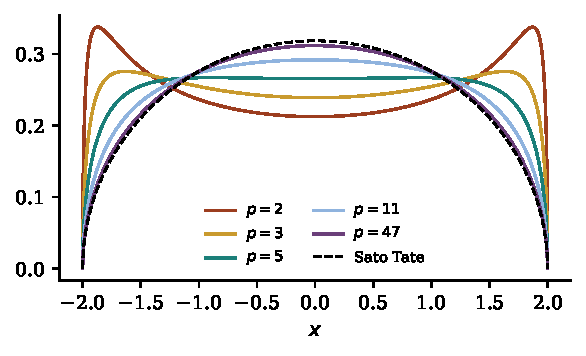
\includegraphics[width=0.85\textwidth]{figs/kestenmckay.pdf}
\caption{Densities of the Kesten McKay laws $\mu_q$ for the primes $q=2,3,5,11,47$ (labelled $p$ in the legend) against the Sato Tate semicircle (dashed). As $q$ grows the mass moves from the edges towards the centre (Theorem~\ref{thm:07tree}(6)).}\label{fig:07kestenmckay}
\end{figure}

\section{Kesten and McKay}

Statement (4) of Theorem~\ref{thm:07tree} can be rewritten as
\[
\Prob(S_{2m}=o)=\rho^{2m}\int\Bigl(\frac x2\Bigr)^{2m}d\mu_q(x),\qquad \rho=\frac{2\sqrt q}{q+1}<1,
\]
and since $\mu_q$ lives on $[-2,2]$ with a density vanishing like a square root at $\pm2$, the integral decays like $m^{-3/2}$. So return probabilities decay like $\rho^n$ up to a polynomial factor. This is Kesten's computation.

\begin{theorem}[Kesten \cite{kesten1959,kesten1959b}]\index{Kesten's theorem}
The spectral radius $\limsup_n\Prob(S_n=o)^{1/n}$ of simple random walk on the $(q+1)$ regular tree is $2\sqrt q/(q+1)$. For a symmetric random walk on a finitely generated group whose step law has finite support generating the group, the spectral radius equals $1$ if and only if the group is amenable.
\end{theorem}

The tree is a Cayley graph of the free product $(\Z/2)^{*(q+1)}$, which is not amenable. Figure~\ref{fig:07treereturn} compares exact return probabilities with $\rho^n$.

\begin{theorem}[McKay \cite{mckay1981}]\index{McKay's law}
Let $G_n$ be $(q+1)$ regular graphs on $n$ vertices such that for every fixed $k$ the number of cycles of length $k$ is $o(n)$. Then the empirical distribution of the eigenvalues of $q^{-1/2}A(G_n)$ converges weakly to $\mu_q$. The hypothesis holds with probability tending to one for uniformly random $(q+1)$ regular graphs.
\end{theorem}

McKay's proof counts closed walks: when short cycles are rare, almost every vertex sees a tree out to any fixed radius, so the empirical moments converge to those of $\mu_q$. In later language the graphs converge locally to the tree in the sense of Benjamini and Schramm \cite{benjaminischramm2001}, and local convergence implies weak convergence of the empirical spectral measures, which are the averages over vertices of the spectral measures at the $\delta_v$.\index{Benjamini Schramm convergence} We use the same argument for the vertical theorem below.

\begin{figure}[t]\centering
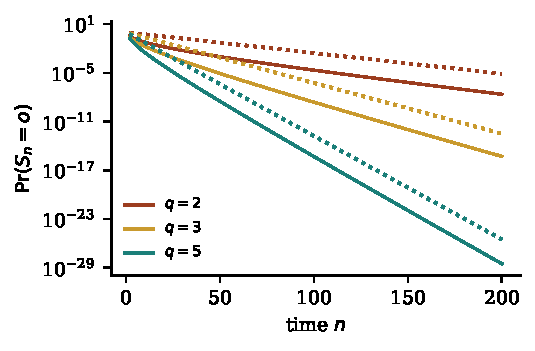
\includegraphics[width=0.7\textwidth]{figs/treereturn.pdf}
\caption{Return probabilities $\Prob(S_n=o)$ of simple random walk on $\T_q$, computed by dynamic programming on the distance chain at even times $n\le200$, for $q=2,3,5$ (solid) against the Kesten rate $(2\sqrt q/(q+1))^n$ (dotted), on a logarithmic scale. Each solid curve lies below its dotted curve by a factor of order $n^{-3/2}$.}\label{fig:07treereturn}
\end{figure}

\section{The $p$ adic Plancherel measure}\index{Plancherel measure}

The spectral theory of $A$ on $\ell^2(\T_q)$ is the spherical harmonic analysis of $\PGL_2(\Q_q)$. An irreducible unramified representation $\pi$ of $\PGL_2(\Q_q)$ has a one dimensional space of $\PGL_2(\Z_q)$ fixed vectors on which $T_q$ acts by a scalar, and by the Satake isomorphism (Theorem~\ref{thm:ch3satake}) this scalar is $q^{1/2}(\alpha+\alpha^{-1})$, where $\{\alpha,\alpha^{-1}\}$ is the Satake parameter, a semisimple conjugacy class in the dual group $\SL_2(\C)$. The representation is tempered exactly when $|\alpha|=1$, that is when $x=\alpha+\alpha^{-1}=2\cos\theta$ lies in $[-2,2]$. Thus
\[
\text{unramified tempered dual of }\PGL_2(\Q_q)\;\longleftrightarrow\;[0,\pi]\;\longleftrightarrow\;[-2,2],
\]
and, with Haar measure normalised so that $\PGL_2(\Z_q)$ has volume one, the Plancherel measure restricted to this set is $\mu_q$: for $\PGL_2(\Q_q)$, Macdonald's Plancherel formula for spherical functions \cite{macdonald1971} is the identity $\langle\delta_o,\phi(X)\delta_o\rangle=\int\phi\,d\mu_q$ with the density of Theorem~\ref{thm:07tree}(3). The nontempered parameters, including the trivial representation at $x=q^{1/2}+q^{-1/2}$ (the pole of the density), carry no Plancherel mass.

The Ramanujan conjecture for $\GL_2$ says that the local components of cuspidal automorphic representations are tempered, so their Satake parameters live in the support of $\mu_q$. For holomorphic forms of weight $k\ge2$ it is Deligne's theorem \cite{deligne1974}, in weight one it is due to Deligne and Serre \cite{deligneserre1974}, and for Maass forms it is open. In the next section the same measure appears as the limiting distribution of these parameters.

\section{The vertical Sato Tate theorem}\index{vertical Sato Tate theorem}

Fix a prime $q$. For $N\ge1$ with $q\nmid N$ and even $k\ge2$, let $x_1,\dots,x_d$ be the eigenvalues, with multiplicity, of $T_q/q^{(k-1)/2}$ on $S_k(\Gamma_0(N))$, where $d=\dim S_k(\Gamma_0(N))$; they lie in $[-2,2]$ by Deligne.

\begin{theorem}[Serre \cite{serre1997}; Conrey, Duke and Farmer \cite{cdf1997}]\label{thm:07serre}
As $k+N\to\infty$ with $k$ even and $q\nmid N$, the empirical measure $d^{-1}\sum_j\delta_{x_j}$ converges weakly to $\mu_q$.
\end{theorem}

Conrey, Duke and Farmer treated level one; Serre treated the general case, including joint equidistribution at finitely many primes.

\paragraph{Proof idea.} For $q\nmid N$ the Hecke relation $T_qT_{q^n}=T_{q^{n+1}}+q^{k-1}T_{q^{n-1}}$ gives $q^{-n(k-1)/2}T_{q^n}=U_n(x/2)$ on an eigenform whose normalised $T_q$ eigenvalue is $x$, the analogue of Exercise~\ref{ex:07hecke}. The Eichler Selberg trace formula expresses $\tr T_{q^n}$ on $S_k(\Gamma_0(N))$ as an identity term, present only for even $n$, plus elliptic terms given by class numbers of imaginary quadratic orders of discriminant $t^2-4q^n$, plus smaller hyperbolic and parabolic terms. After normalisation the identity term divided by the dimension tends to $q^{-n/2}$ for even $n$, and for fixed $n$ the other terms are of lower order than the dimension. Hence $d^{-1}\sum_jU_n(x_j/2)\to\int U_n(x/2)\,d\mu_q$ for every $n$, which gives the vertical law by the method of moments (Theorem~\ref{thm:A:moments}).

The probabilistic reading is cleanest in weight two and prime level $N\equiv1\bmod12$, where the space of forms can be realised on a finite graph. The supersingular $q$ isogeny graph $G_N(q)$ of Chapter~\ref{ch:08} has $h=(N-1)/12$ vertices, is $(q+1)$ regular, and is a finite quotient $\Gamma\backslash\T_q$ of the tree by a discrete cocompact group $\Gamma$ coming from a definite quaternion algebra. Its adjacency eigenvalues are $q+1$ together with those of $T_q$ on $S_2(\Gamma_0(N))$ (Theorem~\ref{thm:08brandt}). Identity (1) of Theorem~\ref{thm:07tree} holds on any $(q+1)$ regular graph, with $A_n$ counting nonbacktracking walks: a step appended to a nonbacktracking walk of length $n$ either extends it to one of length $n+1$ or undoes its last step, and the walks of the second kind number $q$ for each nonbacktracking walk of length $n-1$ ($q+1$ when $n=1$). Taking normalised traces,
\[
\frac1h\sum_{\lambda}\Bigl(U_n\bigl(\tfrac{\lambda}{2\sqrt q}\bigr)-q^{-1}U_{n-2}\bigl(\tfrac{\lambda}{2\sqrt q}\bigr)\Bigr)=\frac{q^{-n/2}}{h}\,\tr A_n ,
\]
which is $q^{-n/2}$ times the expected number of closed nonbacktracking walks of length $n$ from a uniformly random vertex. A closed nonbacktracking walk of length $n$ at a curve $E$ determines, up to sign, an endomorphism of $E$ of degree $q^n$ with cyclic kernel, and by Deuring and Eichler \cite{deuring1941,eichler1954,gross1987} the total number of these over all $E$ is bounded by a sum of class numbers $H(4q^n-t^2)$ that does not depend on $N$. So the right side tends to zero as $N\to\infty$: with probability tending to one, a uniformly random vertex of $G_N(q)$ sees no cycle of bounded length, that is, $G_N(q)$ converges locally to $\T_q$ in the sense of Benjamini and Schramm. The left side is an empirical version of $c_n=q^{-1}c_{n-2}$, and its limit forces the moments of $\mu_q$. In this setting the trace formula is an expectation over a uniformly random vertex of a finite quotient of the tree, its elliptic terms count short cycles, and the vertical theorem is local convergence.

\begin{remark}[Finite level correction]\label{rem:07finite}
The same identity gives the exact finite level bias. The constant eigenvector, with eigenvalue $\lambda=q+1$, contributes $q^{-n/2}(q+1)q^{n-1}/h$ to the left side, where $(q+1)q^{n-1}$ is the size of a sphere of radius $n$ in $\T_q$. Removing it, and writing $x_j=\lambda_j/\sqrt q$ for the $h-1$ normalised nontrivial eigenvalues, the average over the cusp forms is
\[
\frac{1}{h-1}\sum_{j}\Bigl(U_n(x_j/2)-q^{-1}U_{n-2}(x_j/2)\Bigr)=\frac{q^{-n/2}}{h-1}\Bigl(\tr A_n-(q+1)q^{n-1}\Bigr).
\]
For fixed $n$ both terms on the right are $O(1/h)$: the negative one is the Eisenstein contribution, the positive one counts cycles and is class number data. Call the right side $e_n$. If $\hat c_n$ is the average of $U_n(x_j/2)$ over $j$, with $\hat c_{-1}=0$, the left side is $\hat c_n-q^{-1}\hat c_{n-2}$; since $\hat c_0=c_0=1$ and $c_n=q^{-1}c_{n-2}$, induction gives $\hat c_n-c_n=\sum_{0\le k<n/2}q^{-k}e_{n-2k}$, so the balance of the two terms in $e_n,e_{n-2},\dots$ decides the sign of the correction.
\end{remark}

\subsection{Data}

We use the data set of Chapter~\ref{ch:08}, the supersingular $2$ and $3$ isogeny graphs at the $207$ primes $N\equiv1\bmod12$ between $1000$ and $8000$. For $N=1009$ and $q=3$ the nontrivial spectrum agrees with that of $T_3$ on $S_2(\Gamma_0(1009))$ computed by PARI to $10^{-13}$. Pooling the normalised nontrivial eigenvalues $x=\lambda/\sqrt q$ gives $75{,}497$ values for each $q$. Table~\ref{tab:07vertical} compares their Chebyshev averages with $c_n=q^{-n/2}$; the odd averages ($n=1,3$) lie between $-0.0041$ and $-0.0028$ for both $q$. The small deviations are the finite level correction of Remark~\ref{rem:07finite}: for $n=2$ and $q=2$ the deviation is $e_2$, whose pooled Eisenstein term is $-3\cdot207/75497=-0.0082$; the observed deviation is $-0.0040$, and the difference is the positive cycle term. At $n=8$ and $q=3$ the cycle terms win and the average exceeds its limit. Figure~\ref{fig:07vertical} shows the histograms.

\begin{table}[t]\centering\small\setlength{\tabcolsep}{4pt}
\begin{tabular}{lcccccccc}
\toprule
& \multicolumn{4}{c}{$q=2$} & \multicolumn{4}{c}{$q=3$}\\
$n$ & $2$ & $4$ & $6$ & $8$ & $2$ & $4$ & $6$ & $8$\\
\midrule
data & $0.4960$ & $0.2443$ & $0.1194$ & $0.0573$ & $0.3299$ & $0.1071$ & $0.0360$ & $0.0145$\\
$q^{-n/2}$ & $0.5$ & $0.25$ & $0.125$ & $0.0625$ & $0.3333$ & $0.1111$ & $0.0370$ & $0.0123$\\
\bottomrule
\end{tabular}
\caption{Pooled averages of $U_n(x/2)$ over the nontrivial spectra of the supersingular $q$ isogeny graphs at $207$ prime levels, against the tree moments of Theorem~\ref{thm:07tree}.}\label{tab:07vertical}
\end{table}

\begin{figure}[t]\centering
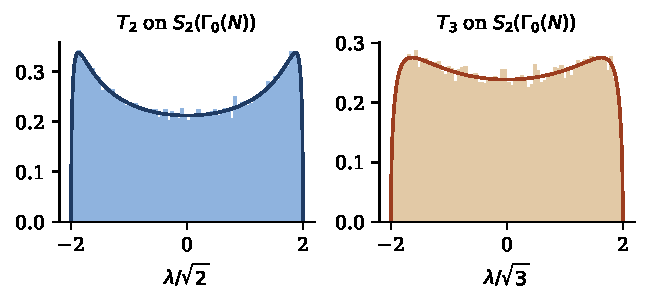
\includegraphics[width=0.9\textwidth]{figs/vertical.pdf}
\caption{Pooled normalised eigenvalues $x=\lambda/\sqrt q$ of $T_2$ (left) and $T_3$ (right) on $S_2(\Gamma_0(N))$ for the $207$ primes $N\equiv1\bmod12$ between $1000$ and $8000$ ($75{,}497$ values for each $q$), computed as nontrivial spectra of supersingular isogeny graphs, against the Kesten McKay densities $\mu_2$ and $\mu_3$.}\label{fig:07vertical}
\end{figure}

\section{Horizontal versus vertical}

There are two limits and two laws. Horizontally, a single newform $f$ without complex multiplication is fixed and $p$ varies; the Satake parameters equidistribute for $\ST$ (Theorem~\ref{thm:04STthm}). Vertically, $q$ is fixed and the form varies over a growing family; the parameters equidistribute for $\mu_q$. Theorem~\ref{thm:07tree}(6) reconciles them. The horizontal statement over primes $p\le x$ samples the local laws $\mu_p$ at ever larger $p$, which by (6) look more and more like the semicircle: the semicircle is the large degree limit of the tree, the free semicircular law of Voiculescu's theory. This is a heuristic for why the two laws are compatible, not a proof of either: the horizontal theorem needs the analytic behaviour of all symmetric power $L$ functions on $\Re s=1$, which comes from their potential automorphy \cite{blght2011}, and the vertical theorem needs the trace formula.

The vertical picture generalises to reductive groups.

\begin{theorem}[Shin \cite{shin2012}]
Let $G$ be a connected reductive group over a totally real field $F$ such that $G(F\otimes_\Q\R)$ has discrete series, under conditions on the centre. For families of cuspidal automorphic representations with level shrinking to the identity at fixed weight, or with weight tending to infinity at fixed level, the normalised counting measures of the local components at a fixed finite place $v$ converge to the Plancherel measure of $G(F_v)$ (tested against the Hecke algebra).
\end{theorem}

For $\PGL_2$ and spherical test functions the weight aspect recovers Theorem~\ref{thm:07serre} at fixed level; the level aspect concerns levels such as those of $\Gamma(N)$, which shrink to the identity, rather than $\Gamma_0(N)$. In higher rank the tree becomes a building, simple random walk becomes several commuting Hecke walks, and $\mu_q$ becomes Macdonald's measure on a torus modulo the Weyl group.

\section{Notes}

The tree of $\PGL_2(\Q_q)$ is constructed in Serre's book \emph{Trees} \cite{serre1980}, which also explains Ihara's theorem that torsion free discrete subgroups of $\SL_2(\Q_q)$ are free \cite{ihara1966}. Kesten's two papers of 1959 \cite{kesten1959,kesten1959b} gave the return probabilities on free groups and the amenability criterion. McKay \cite{mckay1981} found the same law for random regular graphs; Macdonald \cite{macdonald1971} is the reference for spherical functions. The vertical law is due to Serre \cite{serre1997} and, for level one, Conrey, Duke and Farmer \cite{cdf1997}; Sarnak \cite{sarnak1987} had earlier proved the same law for the Hecke eigenvalues of Maass forms on $\SL_2(\Z)$ ordered by Laplace eigenvalue, and Murty and Sinha \cite{murtysinha2009} gave effective versions. Shin's theorem \cite{shin2012} and its quantitative refinement by Shin and Templier \cite{shintemplier2016} put the vertical law in the general setting of the Langlands programme. The individual statements of Theorem~\ref{thm:07tree} are classical, and the recursion for the sphere operators $A_n$ is standard in the theory of Ramanujan graphs \cite{lps1988}; what is ours is the formulation and the single proof organised around the Chebyshev identity (1).

\section{Exercises}

\begin{enumerate}
\item\label{ex:07hecke} Let $T_{q^n}f([L])=\sum f([L'])$, summed over the sublattices $L'\subseteq L$ of index $q^n$, with $T_1=I$. Show that these sublattices are the $q^bL''$ with $0\le b\le n/2$ and $L/L''$ cyclic of order $q^{n-2b}$, so that $T_{q^n}=\sum_{0\le k\le n/2}A_{n-2k}$ on $\T_q$. Show that $T_qT_{q^n}=T_{q^{n+1}}+qT_{q^{n-1}}$ for $n\ge1$, and deduce $q^{-n/2}T_{q^n}=U_n(X/2)$, either from this recursion or by telescoping part (1) of Theorem~\ref{thm:07tree}.
\item Use the density in Theorem~\ref{thm:07tree}(3) and vertex transitivity to show that $\|A\|=2\sqrt q$ on $\ell^2(\T_q)$, and that $\Prob(S_{2m}=o)\sim C_q\,m^{-3/2}\rho^{2m}$; identify $C_q$.
\item Compute the generating function $G(u)=\sum_n\Prob(S_n=o)u^n$ by first passage decomposition of the distance chain and check $G(1)=q/(q-1)$. Show that the radius of convergence of $G$ is $1/\rho$, with branch points at $u=\pm1/\rho$, and relate this to Kesten's theorem.
\item Let $d=d(o,v)$, $U_{-1}=0$ and $U_{-2}=-1$. Show that the function
\[
\varphi_\theta(v)=\tfrac{q}{q+1}q^{-d/2}\bigl(U_{d}(\cos\theta)-q^{-1}U_{d-2}(\cos\theta)\bigr)
\]
satisfies $\varphi_\theta(o)=1$ and $A\varphi_\theta=2\sqrt q\cos\theta\,\varphi_\theta$. For $\theta\in\C$, show that it is bounded exactly when $|\Im\theta|\le\frac12\log q$.
\item Let $\mu_q$ be as in Theorem~\ref{thm:07tree}. Show that $\int\log(4-x^2)\,d\mu_q$ is finite and compute it, using $\log(4\sin^2\theta)=-2\sum_{k\ge1}\cos(2k\theta)/k$ and the Poisson kernel in the proof of (3); compare with $\int\log(4-x^2)\,d\ST=1$.
\end{enumerate}

\section{Open computational problems}

\begin{compproblem}[Rate of vertical convergence]
Objective: measure the rate at which the eigenvalues of $T_p$ on $S_2(\Gamma_0(N))$ approach $\mu_p$, and separate the exact finite level correction from the rest. Data: all primes $N\equiv1\bmod12$ with $37\le N<10^5$ and all primes $p\le50$ with $p\ne N$, so that Remark~\ref{rem:07finite} applies as stated, using PARI/GP \texttt{mfheckemat} for $N\le10^4$ and, beyond, sparse Brandt matrices (Sage or Magma) or supersingular isogeny graphs built as in Chapter~\ref{ch:08}. Deliverable: the Chebyshev averages $\hat c_n(N,p)$ for $n\le20$, split into the Eisenstein and class number terms of Remark~\ref{rem:07finite}, and the Kolmogorov distance to $\mu_p$ as a function of $N$, compared with the effective bounds of Murty and Sinha \cite{murtysinha2009}. Why it matters: each Chebyshev average is given exactly by the trace formula, but the Kolmogorov distance involves all $n$ at once and has no closed form; its decay, and its fluctuation from level to level, can be compared with random matrix heuristics for families (Chapter~\ref{ch:06}).
\end{compproblem}

\begin{compproblem}[Noncongruence quotients]
Objective: compare quotients of the tree by congruence and by noncongruence subgroups of one arithmetic lattice. For a prime $q\equiv1\bmod4$ the lattice $\Gamma\subset\PGL_2(\Q_q)$ of Lubotzky, Phillips and Sarnak \cite{lps1988}, built from integral Hamilton quaternions of norm a power of $q$, is free on $(q+1)/2$ generators and acts simply transitively on the vertices of $\T_q$. A subgroup of index $n$ is therefore given by a transitive action of these generators on $n$ points, and its quotient of $\T_q$ is the $(q+1)$ regular Schreier graph of that action. Data: $q=5$ and $q=13$; congruence subgroups of index up to $10^3$, such as the stabilisers of points of $\mathbb P^1(\mathbb F_M)$ under reduction of $\Gamma$ modulo odd primes $M\ne q$; for each such index, $100$ transitive actions by independent uniform random permutations, which define noncongruence subgroups with probability tending to one (GAP or Magma). Algorithm: sparse eigensolvers and $10^6$ simulated walks per graph up to time $200$. Deliverable: histograms against $\mu_q$, the largest nontrivial eigenvalue against $2\sqrt q$, and return probability curves against Figure~\ref{fig:07treereturn}. Why it matters: congruence quotients are Ramanujan by the Ramanujan bound for weight two forms, while random quotients are only nearly Ramanujan (Friedman \cite{friedman2008}); local convergence to the tree is a property of the graph, the Ramanujan property is arithmetic, and the experiment measures the gap between the two.
\end{compproblem}

\begin{compproblem}[Plancherel statistics for $\GL_3$]
Objective: test Shin's theorem in rank two. Data: quotients of the building of $\PGL_3(\Q_2)$ by cocompact arithmetic lattices, up to $10^5$ vertices, with the two commuting Hecke operators on vertices. Such lattices come from unitary groups in three variables over $\Q$ that are compact at infinity and attached to an imaginary quadratic field in which $2$ splits, so that at $2$ the projective unitary group becomes $\PGL_3(\Q_2)$. Algorithm: for the unitary group of a definite hermitian form, enumerate the genus of a hermitian lattice and compute the Hecke operators by neighbour methods (Magma), diagonalise both, and map joint eigenvalues to Satake parameters in the maximal torus of $\SU(3)$. Deliverable: histograms on the Weyl alcove against Macdonald's Plancherel density, moments of $\SU(3)$ characters, and the proportion of nontempered parameters. Why it matters: it is the first case in which the tree becomes a building, and the Ramanujan property of a quotient is no longer automatic: in Rogawski's classification of the automorphic representations of unitary groups in three variables, the endoscopic lifts of one dimensional representations have nontempered unramified local components and do occur, so the naive Ramanujan conjecture fails for general lattices of this kind, although the bound is known for all other infinite dimensional representations; the proportion of nontempered parameters detects these lifts and measures how far the quotients are from Ramanujan complexes.
\end{compproblem}
